\documentclass[a4paper]{article}

% LaTeX preambule: loading relevant packages, configuring Python listings
\usepackage{graphicx}
\usepackage{amsmath}
\usepackage{color}
\usepackage{listings}
\usepackage{hyperref}
\usepackage{graphicx}
\usepackage{epstopdf}
\usepackage{inputenc}
\usepackage{bm}
\usepackage{physics}
\usepackage{subcaption}
\usepackage{tabto}
\usepackage{multirow}
\def\signed#1{{\unskip\nobreak\hfil\penalty50
    \hskip2em\hbox{}\nobreak\hfil\sl#1
    \parfillskip=0pt \finalhyphendemerits=0 \par}}
\usepackage[a4paper, total={7in, 9in}]{geometry}

\title{%
  Understanding Optical Diffraction and Interference Patterns \\through a Historical Perspective}
\author{PH2255 Final Report\\ \\Candidate 2104412}

\definecolor{dkgreen}{rgb}{0,0.6,0}
\definecolor{gray}{rgb}{0.5,0.5,0.5}
\definecolor{mauve}{rgb}{0.58,0,0.82}

% Settings for colour-coding and formatting Python code:
\lstset{
  language=Python,                % the language of the code
  basicstyle=\footnotesize,           % the size of the fonts that are used for the code
  numbers=left,                   % where to put the line-numbers
  numberstyle=\tiny\color{gray},  % the style that is used for the line-numbers
  stepnumber=5,                   % the step between two line-numbers. If it's 1, each line
                                  % will be numbered
  numbersep=5pt,                  % how far the line-numbers are from the code
  backgroundcolor=\color{white},      % choose the background color. You must add \usepackage{color}
  showspaces=false,               % show spaces adding particular underscores
  showstringspaces=false,         % underline spaces within strings
  showtabs=false,                 % show tabs within strings adding particular underscores
  frame=single,                   % adds a frame around the code
  rulecolor=\color{black},        % if not set, the frame-color may be changed on line-breaks within not-black text (e.g. commens (green here))
  tabsize=2,                      % sets default tabsize to 2 spaces
  captionpos=b,                   % sets the caption-position to bottom
  breaklines=true,                % sets automatic line breaking
  breakatwhitespace=false,        % sets if automatic breaks should only happen at whitespace
  title=\lstname,                   % show the filename of files included with \lstinputlisting;
                                  % also try caption instead of title
  keywordstyle=\color{blue},          % keyword style
  commentstyle=\color{dkgreen},       % comment style
  stringstyle=\color{mauve},         % string literal style
  escapeinside={\%*}{*)},            % if you want to add LaTeX within your code
  morekeywords={*,...}               % if you want to add more keywords to the set
}

\begin{document}
\maketitle

\begin{abstract}
Abstract
\end{abstract}
\clearpage
\tableofcontents
\clearpage
\section{Introduction} \label{sec:intro}
To fully understand an optical theory of light---and to understand why diffraction and interference experiments are so important to ir---it is helpful to understand the history of how different theories arose. Today, we have a very good understanding of light as an electromagnetic interaction between the magnetic and electric fields, enabled by Photons---the EM force carrier. It is common knowledge, even in popular culture, that light exhibits both wave-like and particle-like behaviour. However, in the 17\textsuperscript{th} and 18\textsuperscript{th}, the picture wasn't so clear.\cite[\S1.3]{RefWorks:doc:60689ea38f08cf86c9dc700e}

\subsection{A Brief Historical Overview} \label{sub:over}

While ancient philosiphers---such as Pythagoras, Plato, and Asristotle---began the development of theories of light in the Greek Classical period, progress rapidly accelerated in the seventeenth century with the advent of the refracting telescope. As Galileo and Kepler developed their respective telescope systems in the early 1600s, Snel\footnote{Willebrord Snellius, usually known as Snell} re-discovered Sahl's law of refraction. While these laws did accurately describe light moving through media of varying refractive indices, they rely on the assumption that light travels the path which takes the least time. This assumption can be disproven, such as with a spherical mirror, and as such cannot define a fundemental theory of light.

Nonetheless, Snel's law laid the foundations for a rapid development of modern optics. In 1665, at the Royal Society in London, Hooke was one of the first to study the field known today as diffraction and interference, the subject of this report. In his book \emph{Micrographia} \cite{gut:hooke}, the idea of light being vibrations in a medium was first proposed:
\begin{quote}
  \it{
  ``\ldots this motion is propagated every way with equal velocity, whence necessarily every pulse or vibration of the luminous body will generate a Sphere, which will continually increase, and grow bigger, just after the same manner (though indefinitely swifter) as the waves or rings on the surface of the water do swell into bigger and bigger circles about a point of it, where by the sinking of a Stone the motion was begun, whence it necessarily follows, that all the parts of these Spheres undulated through a Homogeneous medium cut the Rays at right angles.''}
  \signed{\emph{---\cite{gut:hooke}}}
\end{quote}
Thus began the wave theory of light. 
\subsection{Newton's Particle Theory} \label{sub:newt}

Towards the end of the 1600s, at the turn of the 18\textsuperscript{th} century, Newton was making his own advances in the field of optics. In his 1704 paper \emph{Opticks} \cite{gut:newt}, he proposed a particle theory of light---initially set forward by Descartes---where light rays are comprised of small discrete particles named ``corpuscules'', hence its name \emph{the corpuscular theory}. His main motivation for choosing a particle theory was the apparent inability of a wave theory to explain rectilinear propagation\footnote{The propensity of light to travel in a straight line in the absence of any interference.}.

Despite the corpuscular theory's ability to describe both rectilinear propagation and polarisation (whereas wave theories ignored the latter), it relied on assumptions that modern physicists would resoundly reject - that the speed of light is infinite, but also that it sped up in denser media. The corpuscular theory also could not explain observations of chromatic abberation in refracting telescopes, a phenomenon which stifled the use of lens telescopes, Newton preffering to develop reflecting telescopes instead. 
\subsection{Huygens' Wave Theory} \label{sub:huyg}
At the same time, over in mainland Europe, Huygens was developing a theory of his own. His theory posited a wave-like description of light, a rapid vibration in a universal plenum. Continuing the developments of Hooke and Fermat before him, he proposed this theory in his 1690 work \emph{Treatise on Light} \cite{gut:huyg}. This theory relied on a medium for light waves to travel through, known as the ``lumeniferous aether''. Unlike Newton's particle theory, the wave theory could explain rectilinear propogation and diffraction effects---as proved by Fresnel---but due to Newton's immense gravitas and respect, his particle theory remained the popular theory amongst academics throughout the 1700s.

Despite many attempts, the lumeniferous aether proved elusive---even Maxwell's famed electromagnetic equations suggested the existance of such an aether. It was not until 1887, when the Michelson–Morley experiment failed to prove its existance through interferometry, that the idea fell from grace, in preference to theories of special relativity that went on to be devised by Einstein in the early 1900s, and eventually the modern wave-particle photon theory in the advent of quantum mechanics.

\subsection{Developing an Optical Theory of Interference and Diffraction}

In spite of this, the wave-theory approximations of light provide us with reasonably accurate results in some scenarios. As the Maxwell equations are fully compatible with light's motion throuhg a medium, the principles proposed by Hooke (as in \S\ref{sub:over}) and used by Huygens in his wave theory serve as accurate approximations of optical interference and diffraction. By using Hooke's spherical propogation of light waves, Huygens and Fresnel developed an analyitical model of wave propogation:

\begin{quote}
  Every point on a propagating wavefront serves as the source of spherical secondary wavelets, such that the wavefront at some later time is the envelope of these wavelets. If the propagating wave has a frequency $\nu$, and is transmitted through the medium at a speed $v_t$, then the secondary wavelets have that same frequency and speed.
  \signed{---\emph{\cite[\S4.4.2]{RefWorks:doc:60689ea38f08cf86c9dc700e}}}
\end{quote}
This principle, first proposed by Huygens then refined by Fresnel as the Huygens-Fresnel principle (later shown by Kirchoff to be a direct consequence of the differential wave equation), was submitted to the French Academy of sciences in 1818 by Fresnel for review. Poisson, a member of the Academy, was particularly critical of wave theories of light, supporting Newton's corpuscular theory. He found a supposed glaring error in the Huygens-Fresnel principle: under certain conditions, the theory predicts the emergence of a bright spot at the center of the shadow of a small disc, and vice versa; a dark spot at the center of a circular aperture. Poisson stated that, as this phenomenon was not commonly observed, the principle could not be correct. However, another member of the academy, Arago, proved these predictions experimentally, leading the phenomenon to be dubbed the ``Poisson spot'', and heralding one of the first major victories of the wave theory of light over Newton's corpuscular theory.

Such investigations into the Huygens-Fresnel principle are redily replicable with modern equipment, especially with lasers. This report will, through experimental analysis of interference and diffraction phenomena, and relation to the wave equation, investigate the ability for the Huygens-Fresnel principle to approximate the observed behaviour of light, and the modern accepted photonic theory.

\section{Experimental Method}

To investigate the Huygens-Fresnel principle, equations can be constructed to describe the pattern observed from various diffraction and interference experiments. In Newton's particle theory, we would expect an intensity pattern observed behind a single or double slit aperture---placed between a coherent light source and an observation plane---to follow the same shape of the aperture. A wave theory---and observed reality---must account for interference between the two slits in a double-slit aperture, or within a narrow slit for a single-slit setup. 

To begin to formulate an expression for interference patterns behind a single and double slit, approximations of the Huygens-Fresnel principle are considered. In the regime where the observation plane is at a considerable distance from the light source---known as the Fraunhofer regime---the Huygens-Fresnel wavefronts are considered to be planar. As the wavefront advances by forming wavelets along the wavefront, which propogate spherically, the wavefront may be considered planar for the entire source--detector distance. When the distance between the source and detector is considerably smaller, the Fresnel regime is used, where the wavefront is considered parabolic. The transition between these regimes emerges from the derivation of the intensity pattern.

\subsection{Single Slit Intensity Derivation} \label{sec:single}
\begin{figure}[h]
  \centerline{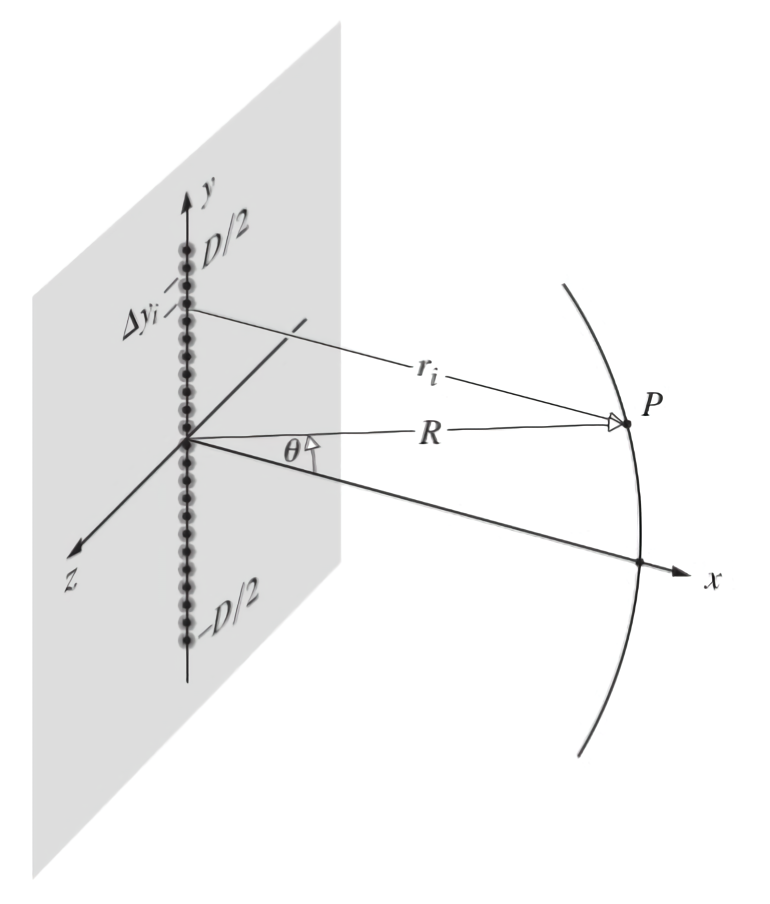
\includegraphics[scale=0.25]{fraunhofer.png}}
  \captionsetup{justification=centering}
  \caption{Illustration of an ideal line-source of electric oscillators on a single-slit \cite[Fig.\ 10.5]{RefWorks:doc:60689ea38f08cf86c9dc700e}}
  \label{fig:fraunhofer}
\end{figure}

To derive an expression for the intensity pattern of a single-slit diffraction experiment, a line of electric oscillation is considered, as shown in Figure~\ref{fig:fraunhofer}. This figure shows a single-slit aperture of width $D$, centered on the origin, and the wavefront propogation at point $P$. Each point on this line emits a spherical wavelet, written as
\begin{equation} \label{eq:oscc}
E=\left(\frac{E_0}r\right)\sin(\omega t-kr)
\end{equation}
where $E_0/r$ is the oscillator's amplitude. In our plane-wavefront approximation in the Fraunhofer regime, $r_i$ in Figure~\ref{fig:fraunhofer} is constant as $y$ varies. The terms of $r$ are expanded to 
\begin{equation} \label{eq:expansion}
  r\approx R-y\sin\theta+\left(\frac{y^2}{2R}\right)\cos^2\theta+\ldots 
\end{equation}
and the non-linear contributions in the third term or greater are negligable as long as its contribution to the phase is insignificant at the edges of the aperture $y=\pm D/2$. From this, a condition of the Fraunhofer regime can be derived, ensuring that $(\pi D^2/4\lambda R)\cos^2\theta$ is negligable, and $r$ is linear with respect to $y$, expressed as
\begin{equation}
  R\gg \frac{\pi x_s^2}\lambda
\end{equation}
where $x_s$ is the significant aperture dimension. The remainder of the terms from Equation \ref{eq:expansion} are substituted into Equation \ref{eq:oscc}, leading to
\begin{equation}
E\approx\left(\frac{E_0}r\right)\sin(\omega t-k[R-y\sin\theta])
\end{equation}
Now, the source strength per unit length $E_L$ is considered, in terms of a change in $y$ of $\Delta y_i$,which allows summation of all of the individual oscillators:
\begin{equation}
E\approx\sum^N_{i=0}\left(\frac{E_L\Delta y_i}{r_i}\right)\sin(\omega t-k[R-y\sin\theta])
\end{equation}
This summation, within the aperture of $y=\pm D/2$, can be converted to an integral, leading to
\begin{equation}
E\approx\frac{E_L}R\int^{+D/2}_{-D/2}\sin(\omega t-k[R-y\sin\theta])
\end{equation}
which by using the substitution of 
\begin{equation} \label{eq:sub}
  \beta\equiv\left(\frac{kD}2\right)\sin\theta =\frac\pi\lambda D\sin\theta
\end{equation}
leads to
\begin{equation}
  E=\frac{E_LD}R\left(\frac{\sin\beta}\beta\right)\sin(\omega t-kR)
\end{equation}
Finally, rewriting this in terms of intensity, with $I(\theta)=\expval{E^2}$, leads to the expression
\begin{equation}
  I(\theta)=\frac12\left(\frac{E_LD}R\right)^2\left(\frac{\sin\beta}\beta\right)^2
\end{equation} where $\expval{\sin^2(\omega t-kR)}=\frac12$. The first two terms can be rewritten as the principal maxiumum, the intensity at $\theta=0$, resulting in
\begin{equation} \label{eq:ss}
I(\theta)=I(0)\frac{\sin^2\beta}{\beta^2}
\end{equation}
as the final expression for the intensity pattern of a single-slit aperture. This describes a $\text{sinc}^2\beta$ pattern that we expect to see from single-slit diffraction, visualised in Figure~\ref{fig:singledemo}.
\begin{figure}[h]
  \centerline{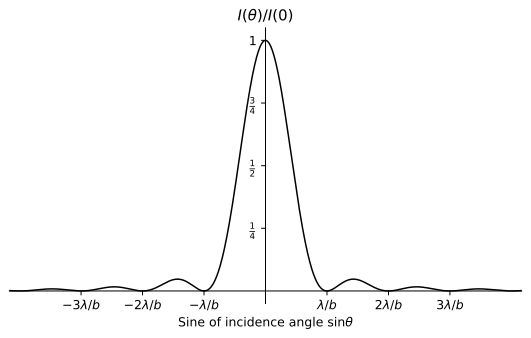
\includegraphics[scale=0.7]{ss_demo.png}}
  \captionsetup{justification=centering}
  \caption{Graph illustrating the general intensity pattern of single-slit diffraction, with light of wavelength $\lambda$, intensity $I$, and slit width $b$}
  \label{fig:singledemo}
\end{figure}

\subsection{Double Slit Intensity Derivation} \label{sec:double}
\begin{figure}[h]
  \centerline{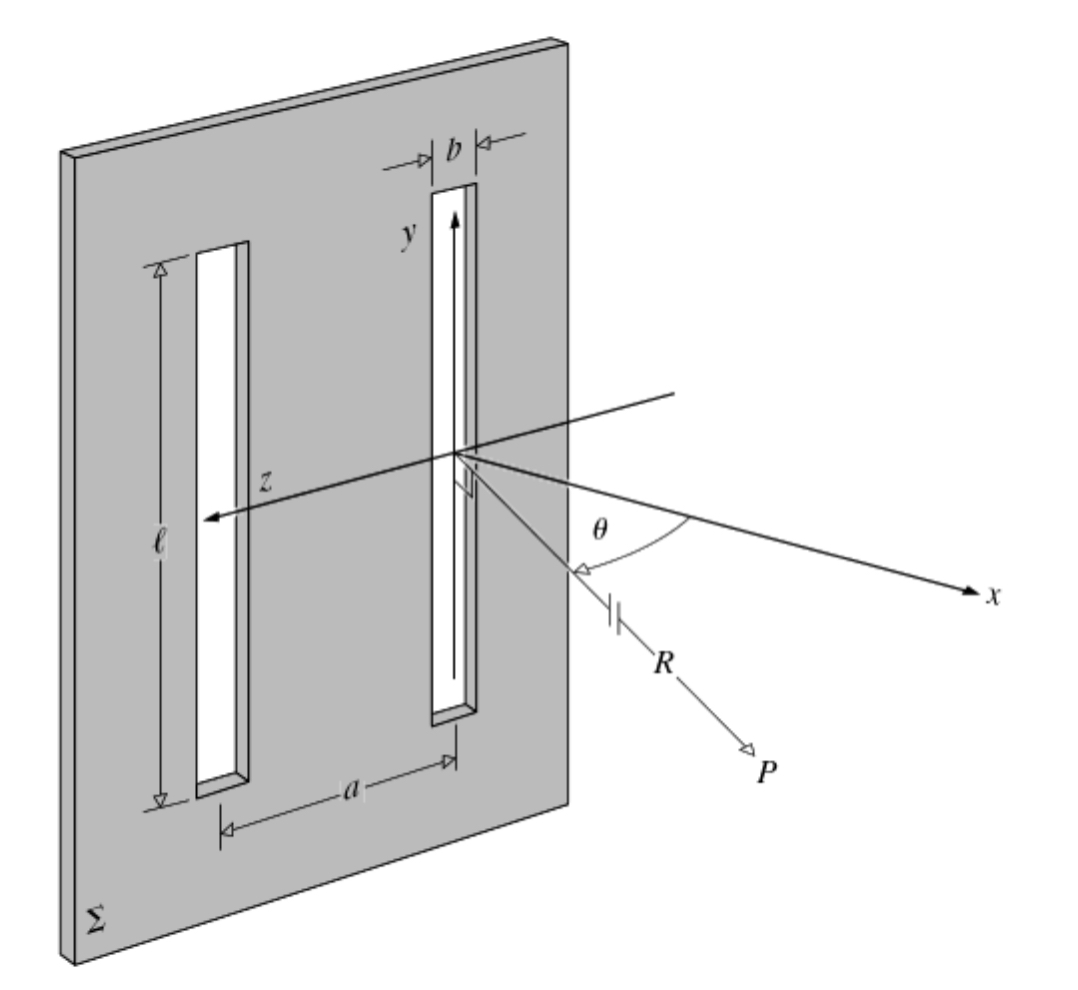
\includegraphics[scale=0.17]{double.png}}
  \captionsetup{justification=centering}
  \caption{Illustration of double-slit diffraction \cite[Fig.\ 10.17]{RefWorks:doc:60689ea38f08cf86c9dc700e}}
  \label{fig:double}
\end{figure}
We can use this same method to obtain the intensity pattern of a double-slit setup, with slight modification. Each of the two slits (of width $b$ and separation $a$) are divided into infinitessimal differential strips ($dz$ by $l$), which behave as point sources along the $z$ axis. Therefore, the total electric field contribution is 
\begin{equation}
E=C\int^{b/2}_{-b/2}F(z)dz+C\int^{a+b/2}_{a-b/2}F(z)dz
\end{equation}
where $F(z)=\sin(\omega t-z[R-z\sin\theta])$, and $C$ is the constant secondary source component. This integration equates to
\begin{equation}
E=bC\left(\frac{\sin\beta}\beta\right)[\sin(\omega t-kR)+\sin(\omega t-kR+2\alpha)]
\end{equation} with the same $\beta\equiv(kb/2)\sin\theta$ as in Equation \ref{eq:sub} (as the single-slit width $D$ equates to the double-slit width $b$), and a new substitution $\alpha\equiv(ka/2)\sin\theta$. This is the summation of the contributions from each slit at the point P, as shown in Figure~\ref{fig:double}. Simplifying this expresison, and squaring it to obtain intensity, we arrive at 
\begin{equation} \label{eq:ds}
I(\theta)=I(0)\left(\frac{\sin^2\beta}{\beta^2}\right)\cos^2\alpha
\end{equation} as a final expression for the intensity pattern of a double-slit. Notice the brackets of this expression; the $\text{sinc}^2$ pattern from the single-slit derivation (Equation \ref{eq:ss}) remains. By plotting Equation \ref{eq:ds}, this is represented by an ``envelope'' of single-slit diffraction, with higher-frequency peaks within it, from the double-slit interference, as seen in Figure~\ref{fig:doubledemo}. It is important to note ``missing maxima''---this occurs when an intensity maxima from the double-slit contribution is ``cancelled out'' by an intensity {\it minima} from the single-slit envelope. This can be observed in Figure~\ref{fig:doubledemo} at the $\lambda/b$ location.

\begin{figure}[h]
  \centerline{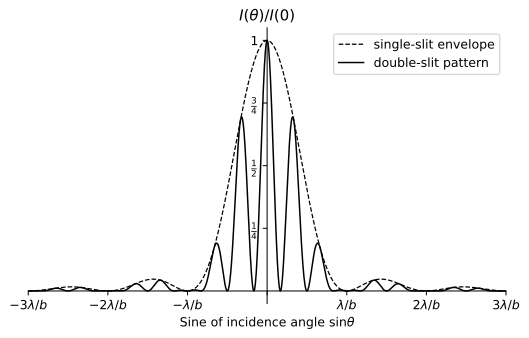
\includegraphics[scale=0.7]{ds_demo.png}}
  \captionsetup{justification=centering}
  \caption{Graph illustrating the general intensity pattern of double-slit diffraction, with light of wavelength $\lambda$, intensity $I$, slit width $b$, and slit separation $a$}
  \label{fig:doubledemo}
\end{figure}

\subsection{Measurements and Data Sets to Obtain}

To investigate the ability of the Huygens-Fresnel principle to approximate the observed behaviour of light, the two expressions Equations \ref{eq:ss} and \ref{eq:ds} can be analysed experimentally. By measuring the maxima and minima positions of the experimental intensity patterns accross a range of slit widths and seperations, the results can be fitted to the predicted curves in the aforementioned equations, and unknown variables determined. As we cannot accurately measure intensity, Equations \ref{eq:ss} and \ref{eq:ds} can be analysed to produce equations for the locations of maxima and minima of the patterns. These locations of maxima and minima are far easier to measure, and still provide a way of determining the either the unknown aperture dimensions, or unknown slit-screen distance.
\clearpage

\section{Experimental Setup}

To analyse the diffraction patterns from a double and single slit, using the expressions derived in Sections \ref{sec:single} and \ref{sec:double}, a very simple experimental setup is used. First, a coherent light source is required. A laser provides a beam of coherent light, at very high directionality, so an incident slit is not require to form a narrow beam line. Secondly, an observation plane is required, to visually analyse the diffraction pattern. This is called a ``Gambrell'' screen, as it has a ruler in millimeters printed to it. Between the two sits the aperture used for the experiment, either the double or single slits, or other apertures such as a pinhole or diffraction grating, which will be discussed later. Figure \ref{fig:setup} illustrates this setup.

\begin{figure}[h]
  \centerline{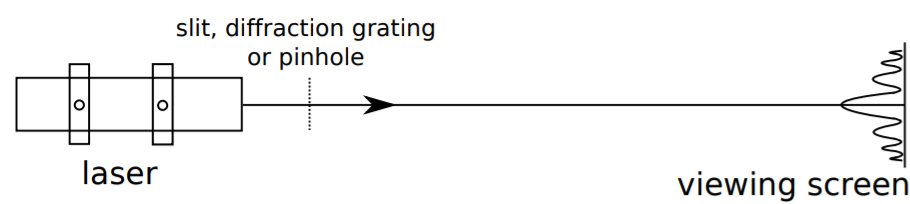
\includegraphics[scale=0.4]{setup.png}}
  \captionsetup{justification=centering}
  \caption{Overhead illustration of the experimental setup used.}
  \label{fig:setup}
\end{figure}

\section{Results}

\subsection{Single Slit Diffraction}

To obtain minima and maxima positions for single-slit diffraction, 8 different slit widths were chosen, and their pattern photographed. Each photograph was then digitally analysed, and the maxima and minima positions annotated and recorded. One example image is displayed in Figure~\ref{fig:ss_measurement} and the rest of the single-slit data is presented in Table \ref{tab:ss_tab}. For the single-slit apertures, the slit-screen distance was measured at $166\pm1$ cm, and the slit width was the unknown variable for each setup. The name for each dataset is derived from the name of the image file given. The maxima and minima positions are recorded with their ``order'', their numerical position away from the center maximum.

\begin{figure}[ht!]
  \centerline{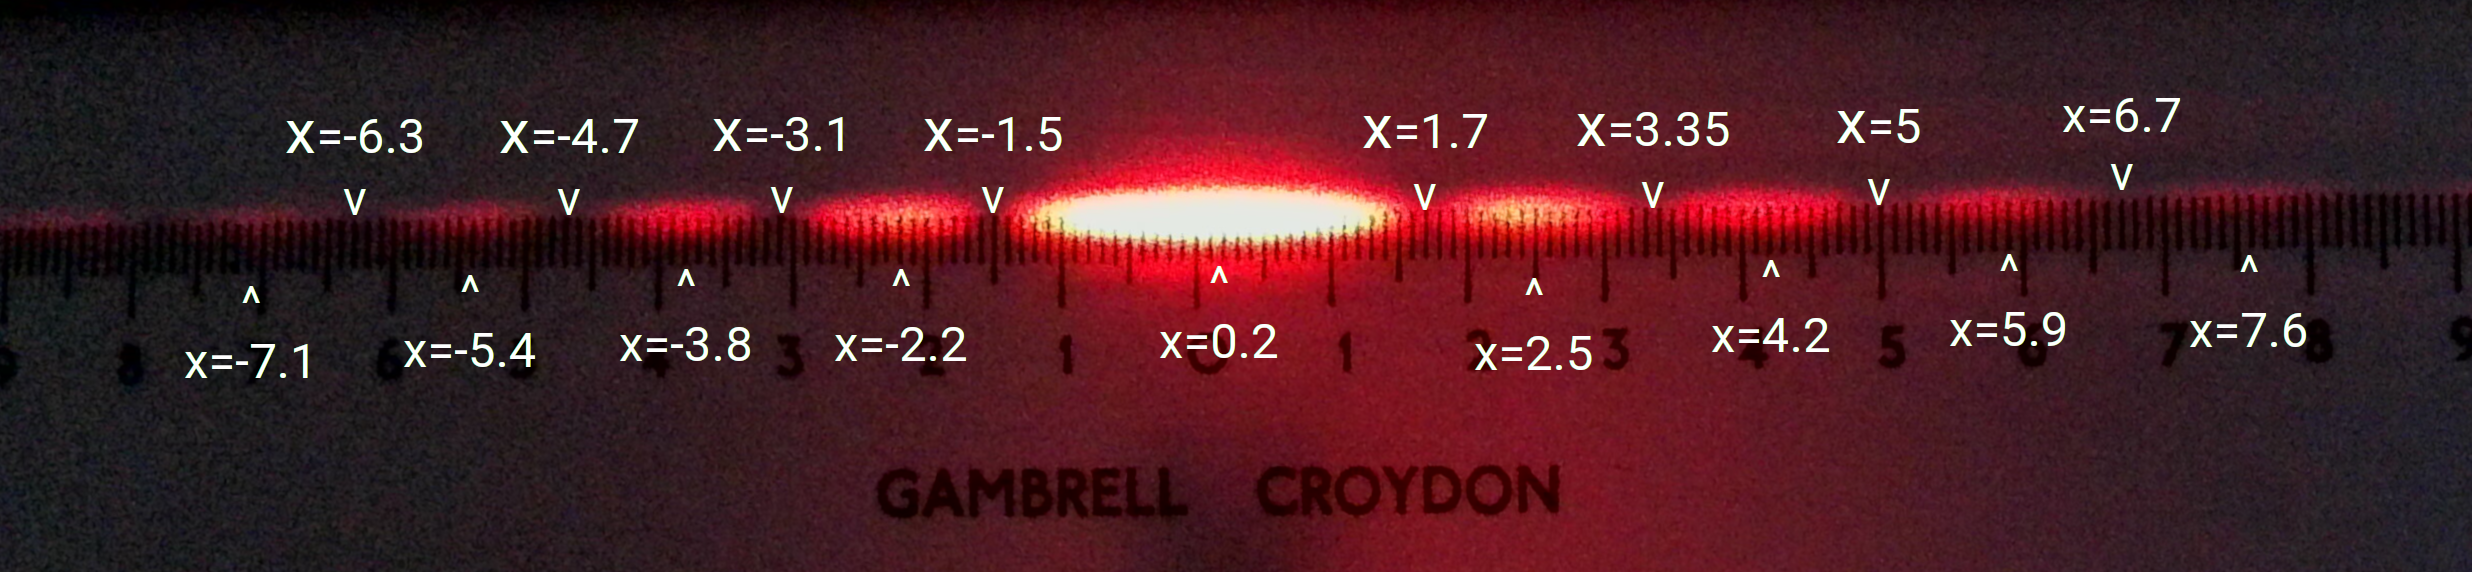
\includegraphics[scale=0.6]{q2sa3.png}}
  \captionsetup{justification=centering}
  \caption{An image of one of the single-slit diffraction patterns measured, edited to include the intensity maxima (indicated at the bottom) and minima locations (indicated at the top).}
  \label{fig:ss_measurement}
\end{figure}

\subsection{Double Slit Diffraction}

Data collection for the double-slit diffraction pattern was identical to that of single-slit patterns, but only 5 data sets were obtained. Due to missing maxima, as noted in Figure~\ref{fig:doubledemo}, it is difficult to accurately measure maxima and minima positions outside the first single-slit envelope. An example image is displayed in Figure~\ref{fig:ds_measurement}, showing the minima above and the maxima below, as well as the area of the first single-slit envelope. The results are tabulated in Table \ref{tab:ds_tab}. For the double-slit apertures, the slit width was measured at $60\mu m$, and the slit seperation at $250\mu m$. The slit-screen distance was the unknown variable for each setup.
\clearpage
\begin{figure}[h]
  \centerline{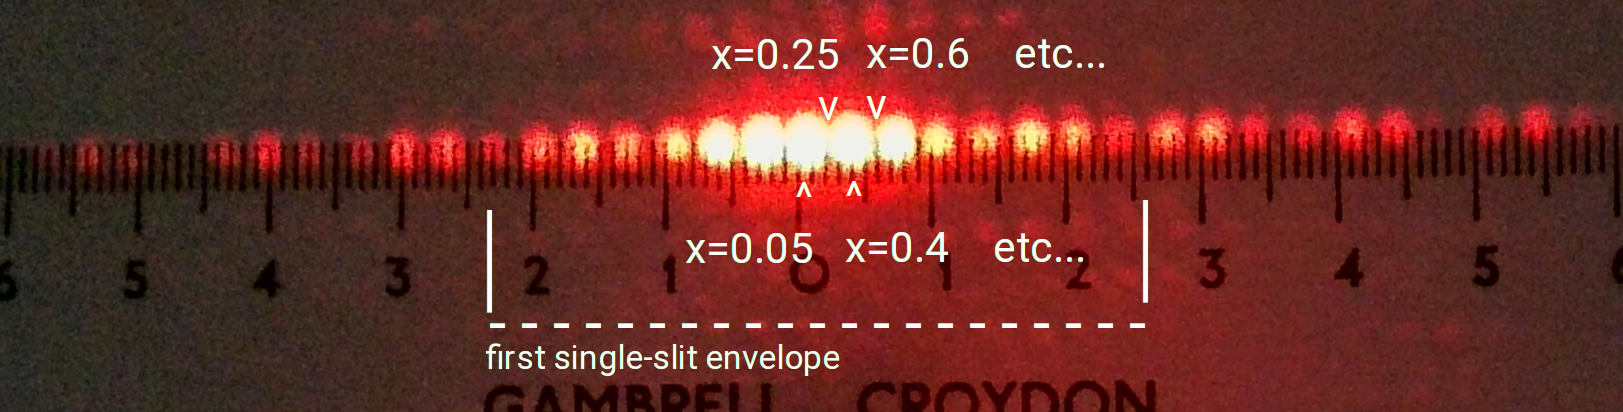
\includegraphics[scale=0.8]{q4ds1.png}}
  \captionsetup{justification=centering}
  \caption{An image of one of the double-slit diffraction patterns measured, edited to include the intensity maxima (indicated at the bottom) and minima locations (indicated at the top), and the first single-slit intensity envelope.}
  \label{fig:ds_measurement}
\end{figure}

\begin{table}[h!]
  \centering
  \begin{tabular}{|c|c|ccccccccc|}
  \hline
  \multirow{2}{*}{Image} & \multirow{2}{*}{Minima/Maxima} & \multicolumn{9}{c|}{Min/Max Position (cm)}               \\
                      &          & -4    & -3    & -2    & -1    & 0    & 1    & 2    & 3    & 4    \\\hline\hline
  \multirow{2}{*}{sa3} & Maxima  & -7.1  & -5.4  & -3.8  & -2.2  & 0.2  & 2.5  & 4.2  & 5.9  & 7.6  \\
                       & Minima  & -6.3  & -4.7  & -3.1  & -1.5  &      & 1.7  & 3.35 & 5    & 6.7  \\\hline
  \multirow{2}{*}{sa4} & Maxima  & -6    & -4.7  & -3.3  & -1.9  & 0.2  & 2.2  & 3.6  & 5.1  & 6.6  \\
                       & Minima  & -5.5  & -4.15 & -2.7  & -1.35 &      & 1.5  & 2.9  & 4.4  & 5.8  \\\hline
  \multirow{2}{*}{sa5} & Maxima  & -5.2  & -4    & -2.8  & -1.6  & 0.1  & 1.9  & 3.1  & 4.3  & 5.6  \\
                       & Minima  & -4.7  & -3.5  & -2.3  & -1.1  &      & 1.3  & 2.5  & 3.7  & 4.9  \\\hline
  \multirow{2}{*}{sb1} & Maxima  & -4.1  & -3.2  & -2.25 & -1.3  & 0.1  & 1.5  & 2.45 & 3.5  & 4.4  \\
                       & Minima  & -3.7  & -2.8  & -2.85 & -0.9  &      & 1.05 & 2    & 2.95 & 3.95 \\\hline
  \multirow{2}{*}{sb2} & Maxima  & -3.75 & -2.9  & -2    & -1.15 & 0.1  & 1.4  & 2.25 & 3.1  & 4    \\
                       & Minima  & -3.35 & -2.5  & -1.65 & -0.8  &      & 0.95 & 1.8  & 2.7  & 3.5  \\\hline
  \multirow{2}{*}{sb3} & Maxima  & -3.3  & -2.55 & -1.8  & -1    & 0.1  & 1.25 & 2    & 2.75 & 3.6  \\
                       & Minima  & -3    & -2.2  & -1.4  & -0.7  &      & 0.9  & 1.3  & 2.4  & 3.2  \\\hline
  \multirow{2}{*}{sb4} & Maxima  & -2.9  & -2.25 & -1.55 & -0.9  & 0.1  & 1.1  & 1.75 & 2.5  & 3.15 \\
                       & Minima  & -2.6  & -1.9  & -1.3  & -0.6  &      & 0.8  & 1.4  & 2.15 & 2.8  \\\hline
  \multirow{2}{*}{sb5} & Maxima  & -2.65 & -2    & -1.4  & -0.8  & 0.15 & 1    & 1.65 & 2.25 & 2.85 \\
                       & Minima  & -2.4  & -1.75 & -1.15 & -0.55 &      & 0.75 & 1.3  & 1.9  & 2.55 \\\hline
  \end{tabular}
  \captionsetup{justification=centering}
  \caption{\label{tab:ss_tab}Tabulated results of single-slit diffraction pattern experiments, for 8 different slit widths.\\ Results are in cenitmeters, with the positional order denoted. All measurements were taken at a slit-screen distance of $116\pm1$ cm, and an error of $\pm 0.05$ cm.}
\end{table}

\begin{table}[h!]
  \centering
  \begin{tabular}{|c|c|ccccccc|}\hline
    \multirow{2}{*}{Image} & \multirow{2}{*}{Minima/Maxima} & \multicolumn{7}{c|}{Min/Max Position (cm)}               \\
    &          & -3    & -2    & -1    & 0    & 1    & 2    & 3      \\\hline\hline
  \multirow{2}{*}{ds1} & Maxima  & -0.9  & -0.6  & -0.25 & 0.05 & 0.4  & 0.75 & 1.05 \\
                       & Minima  & -0.8  & -0.45 & -0.1  &      & 0.25 & 0.6  & 0.9  \\\hline
  \multirow{2}{*}{ds2} & Maxima  & -1.15 & -0.75 & -0.35 & 0    & 0.45 & 0.85 & 1.2  \\
                       & Minima  & -1    & -0.55 & -0.15 &      & 0.25 & 0.65 & 1.05 \\\hline
  \multirow{2}{*}{ds3} & Maxima  & -1.05 & -0.85 & -0.35 & 0.05 & 0.45 & 0.8  & 1.15 \\
                       & Minima  & -0.95 & -0.55 & -0.15 &      & 0.2  & 0.6  & 1    \\\hline
  \multirow{2}{*}{ds4} & Maxima  & -1.35 & -0.9  & -0.4  & 0.05 & 0.5  & 1    & 1.4  \\
                       & Minima  & -1.15 & -0.65 & -0.2  &      & 0.25 & 0.8  & 1.25 \\\hline
  \multirow{2}{*}{ds5} & Maxima  & -1.15 & -0.75 & -0.35 & 0.05 & 0.45 & 0.9  & 1.25 \\
                       & Minima  & -1    & -0.55 & -0.15 &      & 0.25 & 0.7  & 1.1 \\\hline
  \end{tabular}
  \captionsetup{justification=centering}
  \caption{\label{tab:ds_tab}Tabulated results of double-slit diffraction pattern experiments, for 5 different slit widths.\\ Results are in cenitmeters, with the positional order denoted. All measurements were taken with slit width $b\approx 60\mu m$ and slit seperation $a=250\mu m$.}
\end{table}


\section{Data Analysis}

To begin the data analysis, first the maxima position at order 0 was used to cancel the offset of the pattern, and subtracted from each value in that data set. With this adjusted data, it was imported into Python for data manipulation, using Python's \lstinline$NumPy$ library. All code used for the data analysis is found in Appendix \ref{sec:python}, but excerpts are used below. To attempt to verify the Huygens-Fresnel principle, the aim of the data analysis described below is to obtain estimate values for each of the missing variables in each data set.

\subsection{Single Slit} \label{sec:ssan}

For the single-slit data sets, an estimate for the slit width needs to be obtained. To do this, Equation \ref{eq:ss} can be used to derive expressions for the positions of intensity minima and maxima in the $\text{sinc}^2$ pattern. Using the small-angle approximations, the $x$-coordinate of the intensity pattern can be related to its angle $\theta$ with 
\begin{equation} \label{eq:xcoord}
x=L\tan\theta
\end{equation}
where $L$ is the slit-screen distance. Again, we can use Equation \ref{eq:ss} (and, more visually, Figure~\ref{fig:singledemo}) to express the locations of intensity minima as $b\sin\theta=n\lambda$, where $n$ is the minima order as used in Table \ref{tab:ss_tab}, and $b$ is the slit width. By again using the small angle approximation $\sin\theta\approx\tan\theta\approx\theta$, the expression 
\begin{equation} \label{fig:func}
x=L\cdot\frac\lambda{b}n
\end{equation} describes the positions of intensity minima. By once again reffering to Figure~\ref{fig:singledemo}, this same expression can be used to describe the positions of intensity {\it maxima} if each $n$ order is increased absolutely by $\frac12$ (i.e. $n=-1$ becomes $n=-1.5$, $n=2$ becomes $n=2.5$).\\
To fit the data to these expressions, the \lstinline$optimize.curve_fit$ method provided by Python's SciPy library, which uses a method of minimising the sum of the squared residuals to fit a given function to a set of data. Defining \ref{fig:func} as a Python function with \lstinline$_l$ and \lstinline$_w$ as constants for the slit-screen distance $1.66m$ and the laser wavelength $6.238\times10^{-7} m$ as
\begin{lstlisting}[belowskip=-1.5 \baselineskip]
def func(n, *vars):
  a, = vars
  return _l*((_w/a)*n)
\end{lstlisting}
can then be used with NumPy arrays of the $n$ orders, $m$ positions of maxima or minima, and $s$ the uncertainty of $0.05cm$ in each measurement:
\begin{lstlisting}[belowskip=-1.5 \baselineskip]
p0 = np.array([1e-4])
parameters, covariance = curve_fit(func, n, m, p0, s, absolute_sigma=True)
chi_sq_min = sum(((m-func(n, parameters))/s)**2)
\end{lstlisting} 
To determine errors for the calculated values, the standard error propogation formula cannot be used. However, \lstinline$optimize.curve_fit$ also provides the covariance matrix of each fit. The square root of these values is the standard deviation of each result, which can be used as the error in each measurement. 
This snippet also generates a $\chi^2_\text{min}$ value for each data set, which provides a way of quantifying the ``goodness-of-fit'' for each set. The closer that the $\chi^2_\text{min}$ is to the number of degrees of freedom, the better the data fits the calculated fit. Carrying out this fitting to each of the 8 data sets, estimates of the slit width are obtained from the maxima and minima set. Averaging these gives a good estimate. The data and fits for one of the data sets, $\text{sb4}$, are shown in Figure~\ref{fig:ss_ex}, and the full results are tabulated in Table \ref{tab:ss_results}.
\begin{figure}[h]
  \centerline{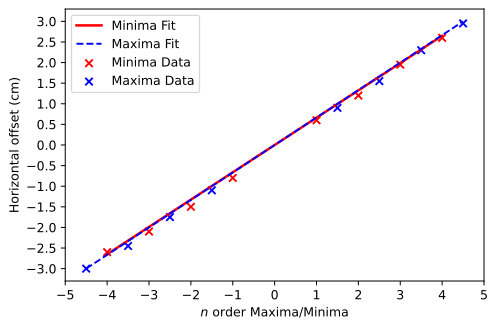
\includegraphics[scale=0.8]{ss_ex.png}}
  \captionsetup{justification=centering}
  \caption{An example of the curve-fitting of a maxima and minima dataset to Equation \ref{fig:func}, using the sb4 dataset.}
  \label{fig:ss_ex}
\end{figure}

\begin{table}[]
  \centering
  \begin{tabular}{|c|cc|cc|c|c|c|}\hline
  \multirow{2}{*}{Data set} & \multicolumn{2}{c|}{Maxima} & \multicolumn{2}{c|}{Minima} & \multirow{2}{*}{$\bar b$ (cm)} & \multirow{2}{*}{$\Delta\bar{b}$ (cm)} & \multirow{2}{*}{$\frac{\chi^2_\text{min}}{\text{NDoF}}$} \\
                       & $b$ (cm) & $\Delta b$ (cm) & $b$ (cm) & $\Delta b$ (cm)   &                     &                      &                      \\\hline\hline
  sa3                    & 0.0064     & 4.76e-10      & 0.00645    & 6.7e-10       & 0.006425            & 5.73e-10             & 0.41035              \\
  sa4                    & 0.00742    & 8.63e-10      & 0.00739    & 1.157e-09     & 0.007405            & 1.01e-09             & 0.50156              \\
  sa5                    & 0.00874    & 1.656e-09     & 0.00873    & 2.253e-09     & 0.008735            & 1.9545e-09           & 0.37458              \\
  sb1                    & 0.011      & 4.161e-09     & 0.01058    & 4.877e-09     & 0.01079             & 4.519e-09            & 5.77901              \\
  sb2                    & 0.01215    & 6.2e-09       & 0.01222    & 8.66e-09      & 0.012185            & 7.43e-09             & 0.59899              \\
  sb3                    & 0.01369    & 9.987e-09     & 0.01387    & 1.4374e-08    & 0.01378             & 1.21805e-08          & 1.10601              \\
  sb4                    & 0.01554    & 1.657e-08     & 0.01563    & 2.3193e-08    & 0.015585            & 1.98815e-08          & 0.59551              \\
  sb5                    & 0.01708    & 2.4176e-08    & 0.01719    & 3.3904e-08    & 0.017135            & 2.904e-08            & 0.59699      \\\hline       
  \end{tabular}
  \captionsetup{justification=centering}
  \caption{Tabulated results of the data analysis for the single-slit diffraction experiment, showing the estimated values for the slit widths for the Maxima and Minima calculations, their average, uncertanties, and $\chi^2_\text{min}$ divided by the number of degrees of freedom in the dataset.}
  \label{tab:ss_results}
  \end{table}

\subsection{Double Slit} \label{sec:dsan}
The data analysis method for double-slit experiments is similar to that of the single-slit analysis. With these data sets, the unknown variable was instead the slit-screen distance, with the slit width $b=60\mu m$ and slit seperation $a=250\mu m$ given. Derivation of expressions for minima positions follow much the same on from Equation \ref{eq:xcoord}. As only minima inside the first single-slit envelope are analysed, only the slit seperation term is required, resulting in a minima condition of 
\begin{equation} \label{eq:func2}
x = l\cdot\frac{\lambda(n+\frac12)}d
\end{equation}\newpage
As with Section \ref{sec:ssan}, this is then written in Python as
\begin{lstlisting}[belowskip=-1.5 \baselineskip]
def func(n, *vars):
    l, = vars
    return l*( (_w/_a)*(n+1/2))
\end{lstlisting} and the same \lstinline$optimize.curve_fit$ method is applied as before. An example of a double-slit fit is shown in Figure~\ref{fig:ds_ex}, and the full results are tabulated in Table~\ref{tab:ds_results}.

\begin{figure}[h]
  \centerline{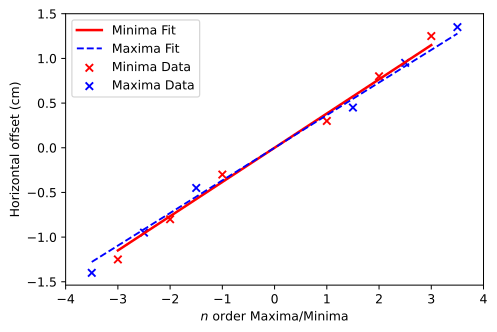
\includegraphics[scale=0.8]{ds_ex.png}}
  \captionsetup{justification=centering}
  \caption{An example of the curve-fitting of a maxima and minima dataset to Equation \ref{eq:func2}, using the ds4 dataset.}
  \label{fig:ds_ex}
\end{figure}

\begin{table}[]
  \centering
  \begin{tabular}{|c|cc|cc|ccc|}
  \hline
  \multirow{2}{*}{Data set} & \multicolumn{2}{c|}{Maxima} & \multicolumn{2}{c|}{Minima} & \multirow{2}{*}{$\bar l$} & \multirow{2}{*}{$\Delta\bar l$} & \multirow{2}{*}{$\frac{\chi^2_\text{min}}{\text{NDoF}}$} \\
                       & $l$ (cm)  & $\Delta l$ (cm)  & $l$ (cm)     & $\Delta l$ (cm) &                     &                      &                      \\\hline\hline
  ds1                    & 104.852      & 9.338       & 103.249      & 13.612      & 104.0505            & 11.475               & 1.48976              \\
  ds2                    & 126.289      & 9.338       & 123.288      & 13.612      & 124.7885            & 11.475               & 1.78767              \\
  ds3                    & 120.697      & 9.338       & 114.457      & 13.612      & 117.577             & 11.475               & 3.47055              \\
  ds4                    & 146.327      & 9.338       & 153.515      & 13.612      & 149.921             & 11.475               & 4.1336               \\
  ds5                    & 128.153      & 9.338       & 125.325      & 13.612      & 126.739             & 11.475               & 2.78745             \\\hline
  \end{tabular}
  \captionsetup{justification=centering}
  \caption{Tabulated results of the data analysis for the double-slit diffraction experiment, showing the estimated values for the slit-screen distance for the Maxima and Minima calculations, their average, uncertanties, and $\chi^2_\text{min}$ divided by the number of degrees of freedom in the dataset.}
  \label{tab:ds_results}
  \end{table}

\newpage
\section{Summary of Results and Conclusion}



\newpage
\begin{appendix}
\section{Appendix}
\subsection{Bibliography}
\emph{All works sourced from the Gutenberg Project are in the public domain.}
\bibliographystyle{plainnat}
\bibliography{export}
\subsection{Python Code}\label{sec:python}
%\lstinputlisting[language=Python,frame=single]{py.py}%

\end{appendix}

\end{document}
